\section*{ÔN TẬP KIỂM TRA CUỐI KÌ 1 - ĐỀ 03}
\setcounter{ex}{0}\setcounter{bt}{0}
\noindent{\bf\fontfamily{qag}\selectfont\color{violet}A. PHẦN TRẮC NGHIỆM}
\Opensolutionfile{ans}[ans/ansBTTeX3]

\begin{ex}%[0D3B2-4]
Nghiệm của phương trình $\sqrt{x-1}=\left(\sqrt{3-x}\right)^2$ là
\choice
{$x=2;x=5$}
{\True $x=2$}
{$x=1;x=3$}
{$x=-1;x=-3$}
\loigiai{
Ta có
\allowdisplaybreaks
\begin{eqnarray*}
\sqrt{x-1}=\left(\sqrt{3-x}\right)^2    &\Rightarrow & \sqrt{x-1}=3-x\\
& \Rightarrow  & x-1=(3-x)^2 \\
& \Rightarrow & x^2-7x+10=0\\
&\Rightarrow & \hoac{&x=2\\&x=5}.
\end{eqnarray*}
Chỉ có nghiệm $x=2$ thỏa mãn phương trình ban đầu. \\
Vậy $S=\{2\}$.
}
\end{ex}

\begin{ex}%[Lê Minh Thiện Anh, Dự án BG10-Lần2]%[0H1Y2-1]
Khẳng định nào sau đây là {\bf sai}?
\choice
{\True Tổng của hai véc-tơ đối nhau bằng 0}
{Véc-tơ-không cùng hướng với mọi véc-tơ}
{Hai véc-tơ đối nhau là hai véc-tơ ngược hướng và cùng độ dài}
{Hai véc-tơ cùng hướng thì chúng cùng phương}
\loigiai{
Tổng của hai véc-tơ đối nhau bằng véc-tơ-không.
}
\end{ex}

\begin{ex}%[Phan Anh]%[0D2B1-3]
Xét sự biến thiên của hàm số $f(x)=x+\dfrac{1}{x}$ trên khoảng $\left(1;+\infty \right)$. Khẳng định nào sau đây đúng?
\choice
{\True Hàm số đồng biến trên khoảng $\left(1;+\infty \right)$}
{Hàm số nghịch biến trên khoảng $\left(1;+\infty \right)$}
{Hàm số vừa đồng biến, vừa nghịch biến trên khoảng $\left(1;+\infty \right)$}
{Hàm số không đồng biến, cũng không nghịch biến trên khoảng $\left(1;+\infty \right)$}
\loigiai{
Ta có
$f\left(x_1\right)-f\left(x_2\right)=\left(x_1+\dfrac{1}{x_1}\right)-\left(x_2+\dfrac{1}{x_2}\right)=\left(x_1-x_2\right)+\left(\dfrac{1}{x_1}-\dfrac{1}{x_2}\right)=\left(x_1-x_2\right)\left(1-\dfrac{1}{x_1x_2}\right).$\\
Với mọi $x_1, x_2\in \left(1;+\infty \right)$ và $x_1<x_2$. Ta có $\heva{
& x_1>1 \\
& x_2>1 \\}\Rightarrow x_1\cdot x_2>1\Rightarrow \dfrac{1}{x_1\cdot x_2}<1.$\\
Suy ra $\dfrac{f\left(x_1\right)-f\left(x_2\right)}{x_1-x_2}=1-\dfrac{1}{x_1x_2}>0\Rightarrow f(x)$ đồng biến trên $\left(1;+\infty \right)$.}
\end{ex}

\begin{ex}%[VanLo HoaTrung, du an tex hoa tai lieu 10]%[0D4Y4-1]
Trong các cặp số sau đây, cặp nào thuộc nghiệm của bất phương trình: $x-4y+5>0$?
\choice
{$(-5;0)$}
{$(-2;1)$}
{\True $(0;0)$}
{$(1;3)$}
\loigiai{
\begin{itemize}
\item Thay tọa độ điểm $(-5;0)$ vào bất phương trình ta được $-5-4.0+5>0$ (sai);
\item Thay tọa độ điểm $(-2;1)$ vào bất phương trình ta được  $-2-4.1+5>0$ (sai);
\item Thay tọa độ điểm $(0;0)$ vào bất phương trình ta được $0-4.0+5>0$ (đúng);
\item Thay tọa độ điểm $(1;3)$ vào bất phương trình ta được $1-4.3+5>0$ (sai).
\end{itemize}
}
\end{ex}

\begin{ex} %[0D1Y2-2]
Trong các khẳng định sau. Hãy chọn khẳng định đúng?
\choice
{$\varnothing \subset \{\varnothing \}$}
{\True $\varnothing \subset \varnothing$}
{$\varnothing \in \varnothing$}
{$\{\varnothing\}\in \{\varnothing \}$}
\loigiai{}
\end{ex}

\begin{ex}%[0H2B1-2]
Tính giá trị biểu thức $P=\cos 30^\circ\cos 60^\circ-\sin 30^\circ\sin 60^\circ$.
\choice
{$P=\sqrt{3}$}
{$P=\dfrac{\sqrt{3}}{2}$}
{$P=1$}
{\True $P=0$}
\loigiai
{Vì $30^\circ$ và $60^\circ$ là hai góc phụ nhau nên $\heva{& \sin 30^\circ=\cos 60^\circ \\
& \sin 60^\circ=\cos 30^\circ \\
}$.\\
$\Rightarrow P=\cos 30^\circ\cos 60^\circ-\sin 30^\circ\sin 60^\circ=\cos 30^\circ\cos 60^\circ-\cos 60^\circ\cos 30^\circ=0$.}
\end{ex}

\begin{ex}%[0D2Y3-3]
Cho hàm số $y=2 x^2-4x+3$ có đồ thị là parabol $(P)$. Mệnh đề nào sau đây sai?
\choice
{$(P)$ không có giao điểm với trục hoành.}
{$(P)$ có đỉnh là $S(1 ; 1)$}
{$(P)$ có trục đối xứng là đường thẳng $y=1$}
{\True $(P)$ đi qua điểm $M(-1 ; 9)$}
\loigiai{Ta có $y(-1)=2\cdot (-1)^2-4\cdot (-1)+3=9$. Vậy $(P)$ đi qua điểm $M(-1;9)$.
}
\end{ex}

\begin{ex}  19.%[0H2B2-1]
Cho hình bình hành $ABCD$ có $AB=8$ cm, $AD=12$ cm,  góc $ABC$ nhọn và diện tích bằng $54$ cm$^2$.  Tính $\cos\left(\overrightarrow{AB}, \overrightarrow{BC}\right)$.
\choice
{$\cos\left(\overrightarrow{AB}, \overrightarrow{BC}\right)=\dfrac{2\sqrt{7}}{16}$}
{$\cos\left(\overrightarrow{AB}, \overrightarrow{BC}\right)=-\dfrac{2\sqrt{7}}{16}$}
{$\cos\left(\overrightarrow{AB}, \overrightarrow{BC}\right)=\dfrac{5\sqrt{7}}{16}$}
{\True $\cos\left(\overrightarrow{AB}, \overrightarrow{BC}\right)=-\dfrac{5\sqrt{7}}{16}$}
\loigiai{
\immini{
Ta có $S_{ABCD}=AB\cdot AD\cdot \sin \widehat{BAD}=54\Rightarrow \sin \widehat{BAD}=\dfrac{9}{16}$\\
$\Rightarrow \cos \widehat{BAD}=-\sqrt{1-\left(\sin \widehat{BAD}\right)^2}=-\dfrac{5\sqrt{7}}{16}$ (do $\widehat{BAD}$ tù).\\
Vậy $\cos\left(\overrightarrow{AB}, \overrightarrow{BC}\right)=\cos \left(\overrightarrow{AB}, \overrightarrow{AD}\right)=\cos \widehat{BAD}=-\dfrac{5\sqrt{7}}{16}$.
}
{
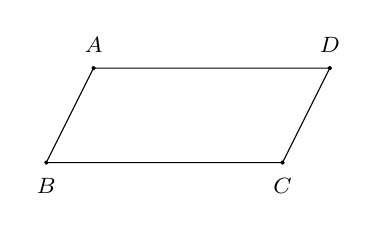
\begin{tikzpicture}[scale=0.6, font=\footnotesize, line join=round, line cap=round, >=stealth]
%Hình 1
\path (0,0) coordinate(A)
(-1,-2) coordinate(B)
(4,-2) coordinate(C)
(5,0) coordinate(D)
;
\foreach \p/\g in {A/90, B/-90, C/-90, D/90}
\draw[fill=black] (\p) circle(1pt) node [shift={(\g:.3)}] {$\p$};
\draw (A)--(B)--(C)--(D)--cycle;
\end{tikzpicture}
}
}
\end{ex}

\begin{ex}%[Đoàn Minh Tân]%[0D4Y5-1]
Bảng xét dấu nào dưới đây là của tam thức $f(x)=-x^2+6x-9$?
\choice
{
\begin{tikzpicture}
\tkzTabInit[nocadre=false, lgt=1.5, espcl=1.5]
{$x$ /0.6,$f(x)$ /0.6}
{$-\infty$,$3$, $+\infty$}
\tkzTabLine{,+,0,-}
\end{tikzpicture}
}
{
\begin{tikzpicture}
\tkzTabInit[nocadre=false, lgt=1.5, espcl=1.5]
{$x$ /0.6,$f(x)$ /0.6}
{$-\infty$,$3$, $+\infty$}
\tkzTabLine{,-,0,+}
\end{tikzpicture}
}
{\True 
\begin{tikzpicture}
\tkzTabInit[nocadre=false, lgt=1.5, espcl=1.5]
{$x$ /0.6,$f(x)$ /0.6}
{$-\infty$,$3$, $+\infty$}
\tkzTabLine{,-,0,-}
\end{tikzpicture}
}
{
\begin{tikzpicture}
\tkzTabInit[nocadre=false, lgt=1.5, espcl=1.5]
{$x$ /0.6,$f(x)$ /0.6}
{$-\infty$,$3$, $+\infty$}
\tkzTabLine{,+,0,+}
\end{tikzpicture}
}
\loigiai{
Tam thức $f(x)=-x^2+6x-9$ có $\Delta=0$, nghiệm kép $x=3$ và hệ số $a=-1<0$ nên có bảng xét dấu như sau
\begin{center}

\begin{tikzpicture}
\tkzTabInit[nocadre=false, lgt=1.5, espcl=1.5]
{$x$ /0.6,$f(x)$ /0.6}
{$-\infty$,$3$, $+\infty$}
\tkzTabLine{,-,0,-}
\end{tikzpicture}
\end{center}
}
\end{ex}

\begin{ex}%[0D3B2-4]
Tập nghiệm của phương trình $\sqrt{2x^2-3}=x-1$ là
\choice
{$\left\{-1-\sqrt{5};-1+\sqrt{5}\right\}$}
{$\left\{-1-\sqrt{5}\right\}$}
{\True $\left\{-1+\sqrt{5}\right\}$}
{$\varnothing$}
\loigiai{
Trước hết ta giải bất phương trình $x-1\geq 0\Leftrightarrow x\geq 1.\; (*)$
\allowdisplaybreaks
\begin{eqnarray*}
&&\sqrt{2x^2-3}=x-1\\
&\Rightarrow&2x^2-3=(x-1)^2\\
&\Rightarrow&x^2+2x-4=0\\
&\Rightarrow&\hoac{&x=-1-\sqrt{5}\\&x=-1+\sqrt{5}.}
\end{eqnarray*}
Trong hai giá trị trên, chỉ có $x=-1+\sqrt{5}$ thỏa mãn $(*)$.\\
Vậy phương trình đã cho có tập nghiệm $S=\left\{-1+\sqrt{5}\right\}$.
}
\end{ex}

\begin{ex}%[Trần Minh,Chuyển sách Tex - 10, 11 (dự án 3)]%[0H1B3-1]
Cho tam giác $ABC$ vuông tại $A$, $M$ là trung điểm của $BC$. Khẳng định nào sau đây đúng?
\choice
{$\overrightarrow{AM}=\overrightarrow{MB}=\overrightarrow{MC}$}
{$\overrightarrow{MB}=\overrightarrow{MC}$}
{\True $\overrightarrow{MB}=-\overrightarrow{MC}$}
{$\overrightarrow{AM}=\dfrac{\overrightarrow{BC}}{2}$}
\loigiai{
Vì $M$ là trung điểm của $BC$ nên $\overrightarrow{MB}+\overrightarrow{MC}=\overrightarrow{0}\Leftrightarrow \overrightarrow{MB}=-\overrightarrow{MC}$. }
\end{ex}

\begin{ex}%[13]%[Nguyễn Diệu Linh]%[0D1Y1-3]
Phủ định của mệnh đề $``\exists x\in \mathbb{Q}:2x^2-5x+2=0"$ là
\choice
{$\exists x\in \mathbb{Q}:2x^2-5x+2>0$}
{$\exists x\in \mathbb{Q}:2x^2-5x+2\neq 0$}
{\True $\forall x\in \mathbb{Q}:2x^2-5x+2\neq 0$}
{$\forall x\in \mathbb{Q}:2x^2-5x+2=0$}
\loigiai
{
Vì phủ định của mệnh đề $``\exists x\in \mathbb{Q}:2x^2-5x+2=0"$ là $``\forall x\in \mathbb{Q}:2x^2-5x+2\neq 0"$.
}
\end{ex}

\begin{ex}%[0H2Y2-1]
Cho $\overrightarrow{a} $ và $\overrightarrow{b} $ là hai véc-tơ cùng hướng và đều khác $\overrightarrow{0} $. Mệnh đề nào sau đây đúng?
\choice
{\True $\overrightarrow{a} \cdot \overrightarrow{b}=\big| \overrightarrow{a}\big| \cdot \big| \overrightarrow{b}\big| $}
{$\overrightarrow{a} \cdot \overrightarrow{b}=0$}
{$\overrightarrow{a} \cdot \overrightarrow{b}=-1$}
{$\overrightarrow{a} \cdot \overrightarrow{b}=-\big| \overrightarrow{a}\big| \cdot \big| \overrightarrow{b}\big| $}
\loigiai{
Ta có $\overrightarrow{a} \cdot \overrightarrow{b}=\big| \overrightarrow{a}\big| \cdot \big| \overrightarrow{b}\big| \cdot \cos\left(\overrightarrow{a},\overrightarrow{b}\right)$. \\
Do $\overrightarrow{a} $ và $\overrightarrow{b} $ là hai véc-tơ cùng hướng nên $ \left(\overrightarrow{a},\overrightarrow{b}\right)=0^\circ $. \\
Vậy $\overrightarrow{a} \cdot \overrightarrow{b}=\big| \overrightarrow{a}\big| \cdot \big| \overrightarrow{b}\big| $.
}
\end{ex}

\begin{ex}%[02]%[Nguyễn Diệu Linh]%[0D1B1-4]
Trong các câu sau, câu nào là mệnh đề \textbf{đúng}?
\choice
{Nếu $a\ge b$ thì $a^2\ge b^2$}
{\True Nếu $a$ chia hết cho $9$ thì $a$ chia hết cho $3$}
{Nếu em chăm chỉ thì em thành công}
{Nếu một tam giác có một góc bằng $60^\circ $ thì tam giác đó đều}
\loigiai
{
\begin{itemize}
\item Mệnh đề $``$Nếu $a\ge b$ thì $a^2\ge b^2"$ là một mệnh đề sai vì $b\le a < 0$ thì $a^2\le b^2$ .
\item Mệnh đề $``$Nếu $a$ chia hết cho $9$ thì $a$ chia hết cho $3"$ là mệnh đề đúng.\\
Vì $a$ $\vdots$ $9\Rightarrow \heva{&a=9n, n\in \mathbb{Z}\\&9\hspace{0.15cm}\vdots\hspace{0.15cm} 3}\Rightarrow a$ $\vdots$  $3$.
\item $``$Nếu em chăm chỉ thì em thành công$"$ chưa là mệnh đề vì chưa khẳng định được tính đúng, sai.
\item Mệnh đề $``$Nếu một tam giác có một góc bằng $60^\circ $ thì tam giác đó đều$"$ là mệnh đề sai vì chưa đủ điều kiện để khẳng định một tam giác là đều.
\end{itemize}
}
\end{ex}

\begin{ex}%[0D2Y3-1]
Hàm số $y=x^2-4 x+3$ đồng biến trên khoảng nào?
\choice
{$(1 ; 3)$}
{$(-\infty ; 2)$}
{$(-\infty ;+\infty)$}
{\True $(2 ;+\infty)$}
\loigiai{
Hàm số bậc hai có $a=1>0$ và $-\dfrac{b}{2a}=2$ nên có bảng biến thiên:
\begin{center}
\begin{tikzpicture}
\draw[thick](-6,4)--(-6,0) (-7,2.8)--(3,2.8);
\path (-6.5,3.45)node{$x$} (-5.5,3.45)node[]{$-\infty$} (2.5,3.35)node[]{$+\infty$} (-1.45,3.45)node[]{$2$} (-6.55,1)node[]{$y$} (-5.5,2.4)node[]{$+\infty$} (-1.5,0.4)node[]{$-1$} (2.6,2.4)node[]{$+\infty$};
\draw[->] (-5.15,2.12)--(-2.03,0.44); \draw[->](-1.02,0.42)--(2.14,2.31);
\end{tikzpicture}
\end{center}
Vậy hàm số đồng biến trên khoảng $(2;+\infty) $.
}
\end{ex}

\begin{ex}%[Phạm Ánh Thư, sách giảng dạy Toán 10]%[0D4Y4-4]
Điểm $M\left(0;-3\right)$ thuộc miền nghiệm của hệ bất phương trình nào sau đây?
\choice
{\True $\heva{& 2x-y\leq 3\\ & 2x+5y\leq 12x+8}$}
{$\heva{& 2x-y>3\\ & 2x+5y\leq 12x+8}$}
{$\heva{& 2x-y>-3\\ & 2x+5y\geq 12x+8}$}
{$\heva{& 2x-y\leq -3\\ & 2x+5y\geq 12x+8}$}
\loigiai{
Thay toạ độ điểm $M\left(0;-3\right)$ vào hệ bất phương trình $\heva{& 2x-y\leq 3\\ & 2x+5y\leq 12x+8}$ ta có: $\heva{& 3\leq 3\\ & -15\leq 8}$ (đúng).
}

\end{ex}

\begin{ex}%[0D2B3-1]
Cho hàm số $y=x^2-2(m+1)x+3$ (với $m$ là tham số). Trên đoạn $[-2018;2018]$ có bao nhiêu giá trị nguyên của tham số $m$ để hàm số đã cho nghịch biến trên khoảng $(-\infty;-1)$?
\choice
{$2019$}
{$2018$}
{$2021$}
{\True $2020$}
\loigiai{
Ta có $a=1>0 \Rightarrow$ hàm số nghịch biến trên khoảng $\left(-\infty;-\dfrac{b}{2a}\right)$.\\
Để hàm số nghịch biến trên khoảng $(-\infty;-1)$ thì $-1<\dfrac{-b}{2a} \Leftrightarrow -1<\dfrac{2(m+1)}{2} \Leftrightarrow m>-2$. \\
Mà $m \in [-2018;2018]$ nên $m\in (-2;2018]$, do $m\in \mathbb{Z}$ suy ra $m\in \{-1;0;\cdots;2018\}$.\\
Do đó có $2020$ giá trị nguyên $m$ thỏa mãn yêu cầu bài toán.}
\end{ex}

\begin{ex}%[0H2B2-1]
Cho tam giác đều $ABC$ có cạnh bằng $a$. Tính tích vô hướng $\overrightarrow{AB}\cdot\overrightarrow{AC}$.
\choice
{$\overrightarrow{AB}\cdot\overrightarrow{AC}=2a^2$}
{$\overrightarrow{AB}\cdot\overrightarrow{AC}=-\dfrac{a^2\sqrt{3}}{2}$}
{$\overrightarrow{AB}\cdot\overrightarrow{AC}=-\dfrac{a^2}{2}$}
{\True $\overrightarrow{AB}\cdot\overrightarrow{AC}=\dfrac{a^2}{2}$}
\loigiai
{Xác định được góc $(\overrightarrow{AB},\overrightarrow{AC} )$ là góc $\widehat{A}$ nên $(\overrightarrow{AB},\overrightarrow{AC} )=60^\circ$.\\
Do đó $\overrightarrow{AB}\cdot\overrightarrow{AC}=AB\cdot AC\cdot\cos(\overrightarrow{AB},\overrightarrow{AC} )=a\cdot a\cdot \cos60^\circ=\dfrac{a^2}{2}$.}
\end{ex}

\begin{ex}%[0D3B2-4]
Nghiệm của phương trình $x-\sqrt{3x^2-9x+1}=2$ là
\choice
{\True $x=3$}
{$x=-\dfrac{1}{2}$}
{$\hoac{&x=-\dfrac{1}{2}\\&x=3}$}
{$x\in\varnothing$}
\loigiai{Phương trình đã cho được viết lại $\sqrt{3x^2-9x+1}=x-2$.\\
Bình phương hai vế của phương trình trên, ta được
\begin{eqnarray*}
3x^2-9x+1=(x-2)^2\Rightarrow 3x^2-9x+1=x^2-4x+4\Rightarrow 2x^2-5x-3=0\Rightarrow x=3 \ \text{hoặc} \ x=-\dfrac{1}{2}.
\end{eqnarray*}
Thay lần lượt các giá trị trên vào phương trình đã cho, ta thấy $x=3$ thỏa mãn.\\
Vậy nghiệm của phương trình đã cho là $x=3$.
}
\end{ex}

\begin{ex}%[0H1B1-1]
    Cho tứ giác $ ABCD $. Có thể xác định được bao nhiêu vectơ (khác $ \overrightarrow{0} $) có điểm đầu và điểm cuối là các điểm $ A $, $ B $, $ C $, $ D $?
    \choice
    {$ 4 $}
    {$ 8 $}
    {$ 10 $}
    {\True $ 12 $}
    \loigiai{Có thể xác định được 12 vectơ (khác $ \overrightarrow{0} $) có điểm đầu và điểm cuối là các điểm $ A $, $ B $, $ C $, $ D $ là các vectơ $ \overrightarrow{AB} $, $ \overrightarrow{AC} $, $ \overrightarrow{AD} $, $ \overrightarrow{BC} $, $ \overrightarrow{BD} $, $ \overrightarrow{CD} $ và các vectơ đối của chúng.
    }
\end{ex}

\begin{ex}%[Trần Minh,Chuyển sách Tex - 10, 11 (dự án 3)]%[0H1B3-2]
Cho tam giác $ABC$ và một điểm $M$ tùy ý. Mệnh đề nào sau đây đúng?
\choice
{$2\overrightarrow{MA}+\overrightarrow{MB}-3\overrightarrow{MC}=\overrightarrow{AC}+2\overrightarrow{BC}$}
{$2\overrightarrow{MA}+\overrightarrow{MB}-3\overrightarrow{MC}=2\overrightarrow{AC}+\overrightarrow{BC}$}
{\True $2\overrightarrow{MA}+\overrightarrow{MB}-3\overrightarrow{MC}=2\overrightarrow{CA}+\overrightarrow{CB}$}
{$2\overrightarrow{MA}+\overrightarrow{MB}-3\overrightarrow{MC}=2\overrightarrow{CB}-\overrightarrow{CA}$}
\loigiai{
Ta có $2\overrightarrow{MA}+\overrightarrow{MB}-3\overrightarrow{MC}=2\overrightarrow{MC}+2\overrightarrow{CA}+\overrightarrow{MC}+\overrightarrow{CB}-3\overrightarrow{MC}=2\overrightarrow{CA}+\overrightarrow{CB}$.
}
\end{ex}

\begin{ex}%[Trần Minh,Chuyển sách Tex - 10, 11 (dự án 3)]%[0H2Y3-1]
Tam giác $ ABC$ có $ AB=\sqrt{2}$, $AC=\sqrt{3}$ và $ \widehat{C}=45^\circ $. Tính độ dài cạnh $ BC$.
\choice
{$ BC=\sqrt{5}$}
{\True $ BC=\dfrac{\sqrt{6}+\sqrt{2}}{2}$}
{$ BC=\dfrac{\sqrt{6}-\sqrt{2}}{2}$}
{$ BC=\sqrt{6}$}
\loigiai
{Theo định lí hàm cô-sin, ta có\\
$ AB^2=AC^2+BC^2-2\cdot AC\cdot BC\cdot \cos \widehat{C}\Rightarrow {(\sqrt{2} )}^2={(\sqrt{3} )}^2+BC^2-2\cdot \sqrt{3}\cdot BC\cdot \cos 45^\circ $ \\
$ \Rightarrow BC=\dfrac{\sqrt{6}+\sqrt{2}}{2}$.}
\end{ex}

\begin{ex}%[Phạm Ánh Thư, sách giảng dạy Toán 10]%[0D4B4-4]
Phần không tô đậm trong hình vẽ dưới đây, biểu diễn tập nghiệm của hệ bất phương trình nào trong các hệ bất phương trình sau?
\begin{center}
\begin{tikzpicture}[line join=round, line cap=round, >=stealth,font=\footnotesize, scale=0.6]
% Vẽ hệ trục toạ độ
\draw (0,0) node [below right] {$0$};
\draw [->] (-3.5,0)--(3.5,0) node[below]{$x$};
\draw[->] (0,-3.5)--(0,3.5) node[left]{$y$};
\clip(-3.5,-3.5) rectangle (3.5,3.5);
% Vẽ các số trên hai trục
\foreach \x in {-2,2}
\draw[shift={(\x,0)},color=black] (0pt,2pt) -- (0pt,-2pt) node[below] {\footnotesize $\x$};
\foreach \y in {1}
\draw[shift={(0,\y)},color=black] (2pt,0pt) -- (-2pt,0pt)node[left] {\footnotesize $\y$};
%Vẽ đồ thị từng hàm số
\draw[samples=100,smooth,domain=-3.5:3.5,black] plot(\x,{-0.333333333*(\x)-0.6666666666});
\draw[samples=100,smooth,domain=-3.5:3.5,black] plot(\x,{0.5*(\x)});
\draw[dashed] (2,0)--(2,1)--(0,1);
% Vẽ miền nghiệm
\fill[pattern=north east lines,opacity=0.6] plot[domain=-3.5:3.5](\x,{-0.333333333*(\x)-0.6666666666})--plot[domain=3.5:-3.5](\x,{3.5})--cycle;
\fill[pattern=north east lines,opacity=0.6] plot[domain=-3.5:3.5](\x,{0.5*(\x)})--plot[domain=3.5:-3.5](\x,{-3.5})--cycle;
\end{tikzpicture}
\end{center}
\choice
{$\heva{& x-2y\leq 0\\ & x+3y\geq -2}$}
{$\heva{& x-2y>0\\ & x+3y<-2}$}
{\True $\heva{& x-2y\leq 0\\ & x+3y\leq -2}$}
{$\heva{& x-2y<0\\ & x+3y>-2}$}
\loigiai{Lấy điểm $(-3;0)$ thuộc vào miền nghiệm. Do đó, ta chọn phương án $\heva{& x-2y\leq 0\\ & x+3y\leq -2}$.
}

\end{ex}

\begin{ex}%[0H2Y1-1]
Cho $\alpha$ là góc tù. Khẳng định nào sau đây \textbf{đúng}?
\choice
{$\sin \alpha<0$}
{$\cos \alpha>0$}
{\True $\tan \alpha<0$}
{$\cot \alpha>0$}
\loigiai{
Do $\alpha$ là góc tù nên $\sin\alpha>0$, $\cos\alpha<0$, $\tan\alpha<0$ và $\cot\alpha<0$.
}
\end{ex}

\begin{ex}%[0H1Y1-1]
Chọn khẳng định đúng trong các khẳng định sau.
\choice
{vectơ là một đường thẳng có hướng}
{vectơ là một đoạn thẳng}
{\True vectơ là một đoạn thẳng có hướng}
{vectơ là một đoạn thẳng không phân biệt điểm đầu và điểm cuối}
\loigiai{vectơ là một đoạn thẳng có hướng.
}
\end{ex}

\begin{ex}%[0D4B5-2]
Cho các mệnh đề\\
(I) Với mọi $x \in [-1;4]$ thì $-x^2+4x+5 \geq 0$.\\
(II) Với mọi $x \in (-\infty;4) \cup (5;10)$ thì $x^2+9x-10>0$. \\
(III) Với mọi $x \in [2;3]$ thì $x^2-5x+6 \leq 0$.
\choice
{\True Mệnh đề (I) và (III) đúng}
{Chỉ mệnh đề (I) đúng}
{Chỉ mệnh đề (III) đúng}
{Cả ba mệnh đề đều sai}
\loigiai{
\begin{itemize}
\item $-x^2+4x+5 \geq 0 \Leftrightarrow -1 \leq x \leq 5$, suy ra mệnh đề (I) đúng.
\item $x^2+9x-10>0 \Leftrightarrow \hoac{& x>1 \\& x<-10}$, suy ra mệnh đề (II) sai.
\item $x^2-5x+6 \leq 0 \Leftrightarrow 2 \leq x \leq 3$, suy ra mệnh đề (III) đúng.
\end{itemize}
}
\end{ex}

\begin{ex}%[0D1K3-3]
Trong số $50$ học sinh của lớp 10A có $15$ bạn được xếp loại học lực giỏi, $25$ bạn được xếp loại hạnh kiểm tốt, trong đó có $10$ bạn vừa được học sinh giỏi vừa được hạnh kiểm tốt. Khi đó, lớp 10A có bao nhiêu bạn được khen thưởng, biết rằng muốn được khen thưởng bạn đó phải có học lực giỏi hay hạnh kiểm tốt.
\choice
{$20$}
{\True $30$}
{$35$}
{$25$}
\loigiai
{
Từ giả thiết bài toán, ta có:
\begin{itemize}
\item Số các học sinh chỉ có học lực giỏi là $15-10=5$.
\item Số các học sinh chỉ được xếp loại hạnh kiểm tốt là $25-10=15$.
\item Tổng số học sinh có học lực giỏi hoặc hạnh kiểm tốt là $10+5+15=30$.
\end{itemize}
Vậy có $30$ học sinh được khen thưởng.
}
\end{ex}

\begin{ex}%[Đỗ Đường Hiếu - ĐCHT THPT]%[0D1B3-2]
Cho tập $ A=\left\{0;2;4;6;8\right\}$; $ B=\left\{3;4;5;6;7\right\}$. Tập $ A\setminus B$ là
\choice
{$\left\{0;6;8\right\}$}
{\True $\left\{0;2;8\right\}$}
{$\left\{3;6;7\right\}$}
{$\left\{0;2\right\}$}
\loigiai{
Ta có $ A\setminus B=\left\{0;2;8\right\}$.
}
\end{ex}

\begin{ex}%[Trần Minh,Chuyển sách Tex - 10, 11 (dự án 3)]%[0H2Y3-1]
Tam giác $ ABC$ có $ AC=4$, $\widehat{BAC}=30^\circ$, $\widehat{ACB}=75^\circ $. Tính diện tích tam giác $ ABC$.
\choice
{$ S_{\Delta ABC}=8$}
{$ S_{\Delta ABC}=4\sqrt{3}$}
{\True $ S_{\Delta ABC}=4$}
{$ S_{\Delta ABC}=8\sqrt{3}$}
\loigiai
{Ta có $ \widehat{ABC}=180^\circ-(\widehat{BAC}+\widehat{ACB} )=75^\circ =\widehat{ACB}$.\\
Suy ra tam giác $ ABC$ cân tại $ A$ nên $ AB=AC=4$.\\
Diện tích tam giác $ ABC$ là $ S_{\Delta ABC}=\dfrac{1}{2}AB\cdot AC\sin \widehat{BAC}=4$.}
\end{ex}

\begin{ex}%[Trần Quốc, BG10-2022, Nhóm 9]%[0H1Y3-1]
Cho hai vectơ  $\vec{a}$, $\vec{b}$ bất kì và số thực $k$. Ta có $k\left(\vec{a}+\vec{b}\right)$ bằng
\choice
{$\vec{a}+k \vec{b}$}
{\True $k \vec{a}+k \vec{b}$}
{$k \vec{a}-k \vec{b}$}
{$k \vec{a}+\vec{b}$}
\loigiai{
Theo tính chất, ta có $k(\vec{a}+\vec{b})=k \vec{a}+k \vec{b}$.
}
\end{ex}

\begin{ex}%[0H1Y1-3]
Phát biểu nào sau đây đúng?
\choice
{Hai vectơ không bằng nhau thì độ dài của chúng không bằng nhau}
{Hai vectơ không bằng nhau thì độ dài của chúng không cùng phương}
{\True Hai vectơ bằng nhau thì có giá trùng nhau hoặc song song nhau}
{Hai vectơ có độ dài không bằng nhau thì không cùng hướng}
\loigiai{
Hai vectơ bằng nhau thì cùng phương nên chúng có giá trùng nhau hoặc song song nhau.
}
\end{ex}

\begin{ex}%[Đoàn Minh Tân]%[0D4Y5-1]
Tam thức $f(x)=x^2-12x-13$ nhận giá trị âm khi và chỉ khi
\choice
{$x<-13$ hoặc $x>1$}
{$x<-1$ hoặc $x>13$}
{$-13<x<1$}
{\True $-1<x<13$}
\loigiai{
Tam thức $f(x)=x^2-12x-13$ có $\Delta =196>0$, hai nghiệm $x_1=-1$, $x_2=13$ và hệ số $a=1>0$.\\
Bảng xét dấu của $f(x)$ như sau
\begin{center}

\begin{tikzpicture}
\tkzTabInit[nocadre=false, lgt=1.5, espcl=1.5]
{$x$ /0.6,$f(x)$ /0.6}
{$-\infty$,$-1$,$13$, $+\infty$}
\tkzTabLine{,+,0,-,0,+}
\end{tikzpicture}
\end{center}
Do đó $f(x)<0$ khi $-1<x<13$.
}
\end{ex}

\begin{ex}%[Phan Anh]%[0D2B1-1]
Cho hàm số $f(x)=\left\{\begin{array}{*{35}{l}}
\dfrac{2}{x-1} &, x\in(-\infty;0) \\
\sqrt{x+1} &, x\in[0;2] \\
x^2-1 &, x\in(2;5]
\end{array}\right.$. Tính giá trị của $f(4)$.
\choice
{$f(4)=\dfrac{2}{3}$}
{\True $f(4)=15$}
{$f(4)=\sqrt{5}$}
{Không tính được}
\loigiai{Do $4\in(2;5]$ nên $f(4)=4^2-1=15$.}
\end{ex}

\begin{ex}%[Phan Anh]%[0D2B1-2]
Tìm tập xác định $\mathscr{D}$ của hàm số $y=\dfrac{2x+1}{x^3-3x+2}$.
\choice
{$\mathscr{D}=\mathbb{R}\setminus\left\{1;2\right\}$}
{\True $\mathscr{D}=\mathbb{R}\setminus\left\{-2;1\right\}$}
{$\mathscr{D}=\mathbb{R}\setminus\left\{-2\right\}$}
{$\mathscr{D}=\mathbb{R}$}
\loigiai{
Hàm số xác định khi $\begin{aligned}[t]
&x^3-3x+2\ne 0\Leftrightarrow (x-1)(x^2+x-2)\ne 0\\
\Leftrightarrow&\,\heva{
& x-1\ne 0 \\
& x^2+x-2\ne 0}\Leftrightarrow \heva{
& x\ne 1 \\
& \heva{
& x\ne 1 \\
& x\ne-2}}\Leftrightarrow \heva{
& x\ne 1 \\
& x\ne-2.}
\end{aligned}$\\
Vậy tập xác định của hàm số là $\mathscr{D}=\mathbb{R}\setminus\left\{-2;1\right\}$.}
\end{ex}

\begin{ex}%[0-GHK2-2021, THPT Nguyễn Trường Tộ, 2020-2021]%[Vô Văn Tự]%[0D4B4-1]
Cho đường thẳng $d\colon 7x-9y+2=0$ chia mặt phẳng toạ độ làm hai nửa  mặt phẳng, trong đó miền nghiệm của bất phương trình $7x-9y+2>0$ là nửa mặt phẳng
\choice
{có bờ là đường thẳng $d$ và không chứa điểm $O(0;0)$}
{\True không có bờ $d$ và chứa điểm $O(0;0)$}
{có bờ là đường thẳng $d$ và chứa điểm $O(0;0)$}
{không chứa bờ $d$ và không chứa điểm $O(0;0)$}
\loigiai{
Ta có toạ độ điểm $O(0;0)$ thoả mãn bất phương trình $7x-9y+2>0$ nên miền nghiệm của bất phương trình $7x-9y+2>0$ là nửa mặt phẳng không có bờ $d$ và chứa điểm $O(0;0)$.
}
\end{ex}
\Closesolutionfile{ans}

\noindent{\bf\fontfamily{qag}\selectfont\color{violet}B. PHẦN TỰ LUẬN}

\begin{ex}[1,0 điểm]
Vẽ đồ thị hàm số $y=x^2+6x-5$.
\loigiai{
\immini{
Ta có $AC^2+BC^2=AB^2\Leftrightarrow 2AC^2=2\Rightarrow AC=BC=1$.\\
$AM=\sqrt{AC^2+CM^2}=\sqrt{1^2+\left(\dfrac{1}{2}\right)^2}=\dfrac{\sqrt{5}}{2}$.\\
$\left|\overrightarrow{AB}+\overrightarrow{AC} \right| =\left| 2\overrightarrow{AM}\right| =2AM=\sqrt{5}  $.
}{
\begin{tikzpicture}[scale=1,>=stealth]
\tkzDefPoints{0/0/C,3/0/B, 0/3/A}
\tkzDefMidPoint(B,C)\tkzGetPoint{M}
\tkzDrawSegments(A,B B,C B,A A,M A,C)
\tkzLabelPoints[above](A)
\tkzLabelPoints[below](B,C,M)
\tkzDrawPoints[fill=black](A,B,C,M)
\end{tikzpicture}}}
\end{ex}

\begin{ex}[0,5 điểm]%[Hoàng Thanh Phương, BG10-2022-Đợt 2, Nhóm 3]%[0D4B5-1]
Giải bất phương trình sau $-3x^2+7x-4< 0$ bằng cách lập bảng xét dấu.
\loigiai{
Tam thức bậc hai $f(x)=-3x^2+7x-4$ có $a=-3<0$ và có hai nghiệm phân biệt $x_1=1$ và $x_2=\dfrac43$. \\
Suy ra $f(x)< 0$ với mọi $x\in(-\infty;1) \cup \left(\dfrac43;+\infty\right)$. \\
Vậy tập nghiệm của bất phương trình là $S=(-\infty;1) \cup \left(\dfrac43;+\infty\right)$.
}
\end{ex}

\begin{ex}[0,5 điểm]%[Phan Anh]%[Dự án giáo án 10]%[0H1B2-5]
Cho tam giác $ABC$ vuông cân tại $C$, $AB=\sqrt{2}$. Tính độ dài của $\overrightarrow{AB}+\overrightarrow{AC}$.
\loigiai{
\immini{
Ta có $AC^2+BC^2=AB^2\Leftrightarrow 2AC^2=2\Rightarrow AC=BC=1$.\\
$AM=\sqrt{AC^2+CM^2}=\sqrt{1^2+\left(\dfrac{1}{2}\right)^2}=\dfrac{\sqrt{5}}{2}$.\\
$\left|\overrightarrow{AB}+\overrightarrow{AC} \right| =\left| 2\overrightarrow{AM}\right| =2AM=\sqrt{5}  $.
}{
\begin{tikzpicture}[scale=1,>=stealth]
\tkzDefPoints{0/0/C,3/0/B, 0/3/A}
\tkzDefMidPoint(B,C)\tkzGetPoint{M}
\tkzDrawSegments(A,B B,C B,A A,M A,C)
\tkzLabelPoints[above](A)
\tkzLabelPoints[below](B,C,M)
\tkzDrawPoints[fill=black](A,B,C,M)
\end{tikzpicture}}}
\end{ex}

\begin{ex}[0,5 điểm]%[Nguyễn Tất Thu, BG10-2022]%[0H2G2-4]
Cho tam giác $ABC$. Tìm tập hợp điểm $M$ sao cho \[\left( \overrightarrow{MA}+2\overrightarrow{MB}+3\overrightarrow{CB} \right)\overrightarrow{BC}=0.\]
\loigiai{
Gọi $I$ là điểm xác định bởi \[\overrightarrow{IA}+2\overrightarrow{IB}=\overrightarrow{0}.\]
Khi đó \[\begin{aligned}
& \left( \overrightarrow{MA}+2\overrightarrow{MB}+3\overrightarrow{CB} \right)\overrightarrow{BC}=0\\
\Leftrightarrow &\ \left[ \left( \overrightarrow{MI}+\overrightarrow{IA} \right)+2\left( \overrightarrow{MI}+\overrightarrow{IB} \right) \right]\cdot \overrightarrow{BC}=3BC^2 \\
\Leftrightarrow &\ \overrightarrow{MI}\cdot \overrightarrow{BC}=BC^2
\end{aligned}\]
Gọi $M'$, $I'$ lần lượt là hình chiếu của $M$, $I$ lên đường thẳng $BC$. \\
Theo công thức hình chiếu ta có \[\overrightarrow{MI}\cdot \overrightarrow{BC}=\overrightarrow{M'I'}\cdot \overrightarrow{BC}.\] Do đó \[\overrightarrow{M'I'}\cdot \overrightarrow{BC}=BC^2.\]
Vì $BC^2>0$ nên $\overrightarrow{M'I'},\ \overrightarrow{BC}$ cùng hướng suy ra
\[\overrightarrow{M'I'}\cdot \overrightarrow{BC}=BC^2\Leftrightarrow M'I'\cdot BC=BC^2\Leftrightarrow M'I'=BC.\]
Do $I$ cố định nên $I'$ cố định suy ra $M'$ cố định.\\
Vậy tập hợp điểm $M$ là đường thẳng đi qua $M'$ và vuông góc với $BC$.
}
\end{ex}

\begin{ex}[0,5 điểm]%[Đề kiểm tra HK2 môn Toán 10 trường THPT Nguyễn Thượng Hiền]%[Đoàn Minh Tân, 10EX-HK2-2223]%[0D4T5-6]
    \immini{Cho hòn đảo $D$ cách bờ $4$ km ($CD=4$ km). Ngôi làng $B$ cách $C$ một khoảng $7$ km. Nhà nước muốn xây dựng một trạm y tế trên đất liền, sao cho có thể phục vụ được cho dân cư ở cả đảo $D$ và làng $B$. Biết trung bình vận tốc di chuyển chuyến tàu cứu thương là $100$ km/h, xe cứu thương là $80$ km/h. Vậy nên đặt trạm y tế cách đảo $D$ bao xa để thời gian cứu thương cho hai địa điểm là như nhau?
        }
        {\begin{tikzpicture}[scale=.7, font=\footnotesize,line join=round, line cap=round,>=stealth]
                \coordinate (C) at (0,0);
                \coordinate (D) at (0,4);
                \coordinate (A) at (3,0);
                \coordinate (B) at (7,0);
                \draw (B)--(C)--(D)--(A);
                \foreach \i/\j in {A/above,B/below,C/below,D/left}
                \draw[fill=black] (\i) circle(1pt) node[\j]{$\i$};
                \draw[<->] (0,-1)--(3,-1) node[below]{$7$ km}--(7,-1);
                \draw (0,2) node[left]{$4$ km} (D) node[above right]{Hòn đảo} (A) node[below]{Trạm y tế} (B) node[right]{Ngôi làng};
            \end{tikzpicture}
        }   
    \loigiai{
    Đặt $AB=x$ ($0<x<7$), suy ra $AC=7-x$, $AD=\sqrt{CD^2+CA^2}=\sqrt{16+(7-x)^2}$.\\
    Thời gian di chuyển của tàu cứu thương từ $D$ đến $A$ là $\dfrac{\sqrt{16+(7-x)^2}}{100}$.\\
    Thời gian di chuyển của xe cứu thương từ $B$ đến $A$ là $\dfrac{x}{80}$.\\
    Do thời gian cứu thương cho hai địa điểm là như nhau nên ta có phương trình \allowdisplaybreaks
    \begin{eqnarray*}
        &&\dfrac{\sqrt{16+(7-x)^2}}{100}=\dfrac{x}{80}\\
        &\Rightarrow& 4\sqrt{16+(7-x)^2}=5x\\
        &\Rightarrow& 16(65-14x+x^2)=25x^2\\
        &\Rightarrow& 9x^2+224x-1040\\
        &\Rightarrow& \hoac{& x=4\\ & x=-\dfrac{260}{9}.}
    \end{eqnarray*} 
    Thử lại ta nhận $x=4$ (thoả mãn điều kiện).\\
    Vậy trạm y tế đặt cách đảo $D$ một khoảng bằng $\sqrt{16+(7-4)^2}=5$ km.
    }
\end{ex}